% This LaTeX document needs to be compiled with XeLaTeX.
\documentclass[10pt]{article}
\usepackage[utf8]{inputenc}
\usepackage{amsmath}
\usepackage{amsfonts}
\usepackage{amssymb}
\usepackage[version=4]{mhchem}
\usepackage{stmaryrd}
\usepackage{graphicx}
\usepackage[export]{adjustbox}
\graphicspath{ {./images/} }
\usepackage{multirow}
\usepackage[fallback]{xeCJK}
\usepackage{polyglossia}
\usepackage{fontspec}
\setCJKmainfont{Noto Serif CJK TC}

\setmainlanguage{german}
\setmainfont{CMU Serif}

\begin{document}
\section*{Deskriptive Statistik}
\section*{Grundbegriffe}
PMF: $\quad f(x)$ Relative Häufigkeit (Stabdiagramm) CMF: $F(x)$ Kumulative relative Häufigkeit (Treppendiagramm)\\
PDF: $\quad f(x)$ Höhe Balken Histogramm\\
CDF: $F(x)$ Kulutaive Fläche Balken Histogramm\\
$h_{i}: \quad$ Absolute häufigkeit\\
$f_{i}: \quad$ Relative häufigkeit\\
$x_{\text {med }}: \quad 2$. Quantil oder $R_{0.5}$\\
$x_{\text {mod }}$ : Modus oder Modalwert ist der häufigste Stichprobenwert\\
$\bar{x}: \quad$ arithmetisches Mittel\\
$s_{x}^{2}$ : Varianz\\
$s_{x}$ : Standardabweichung\\
$s_{k o r}: \quad$ korrigierte Standardabweichung

\section*{Funktionstypen}
PMF\\
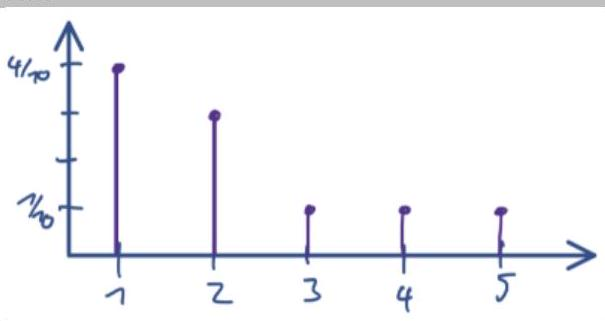
\includegraphics[width=\linewidth]{images/2024_12_29_0906b02acf849bda8665g-1(1)}

CMF\\
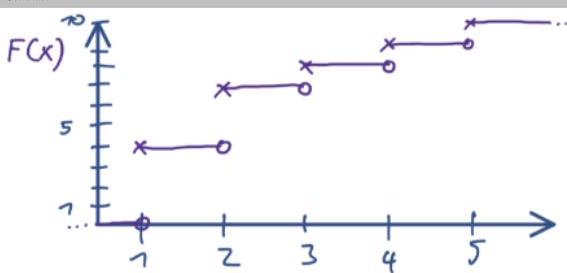
\includegraphics[width=\linewidth]{images/2024_12_29_0906b02acf849bda8665g-1(4)}\\
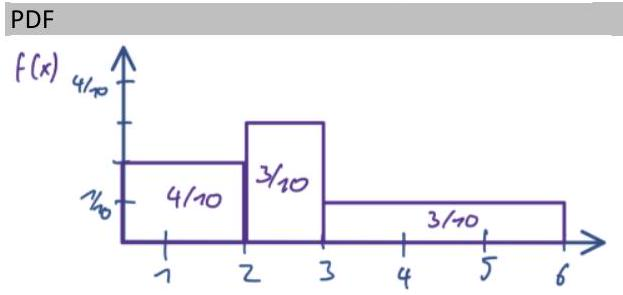
\includegraphics[width=\linewidth]{images/2024_12_29_0906b02acf849bda8665g-1(3)}\\
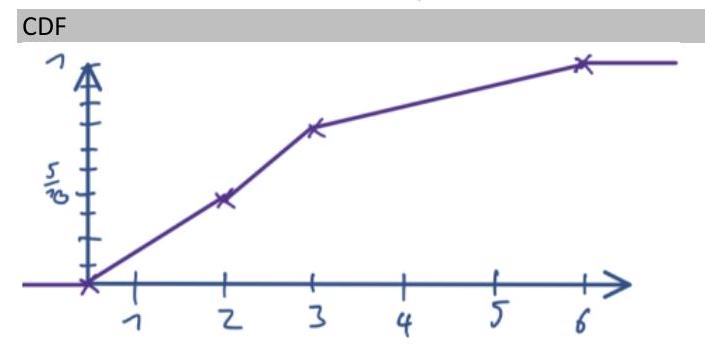
\includegraphics[width=\linewidth]{images/2024_12_29_0906b02acf849bda8665g-1}

Boxplot\\
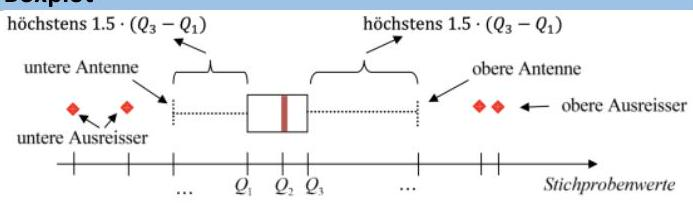
\includegraphics[width=\linewidth]{images/2024_12_29_0906b02acf849bda8665g-1(5)}

Untere und obere Antenne sind Stichprobenwerte! Median bei GERADER Anzahl von Werten\\
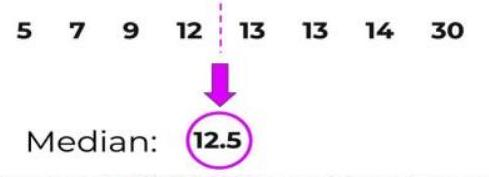
\includegraphics[width=\linewidth]{images/2024_12_29_0906b02acf849bda8665g-1(7)}

Median bei UNGERADER Anzahl von Werten\\
$\begin{array}{llllllllllllllll}5 & 7 & 9 & 12 & 13 & 13 & 14 & 16 & 30\end{array}$

\section*{Eingabe in Taschenrechner}
Lists \& Spreadsheet öffnen\\
Spalte oben beschriften\\
Werte in Spalte eintragen\\
Doc $\rightarrow 4$ Einfügen $\rightarrow 7$ Data \& Statistics\\
Unten auf «Klicken für mehr Variablen» und auswählen Menu $\rightarrow 1$ Plot-Typ $\rightarrow 2$ Box-Plot

\section*{Quantil}
Quantile CDF\\
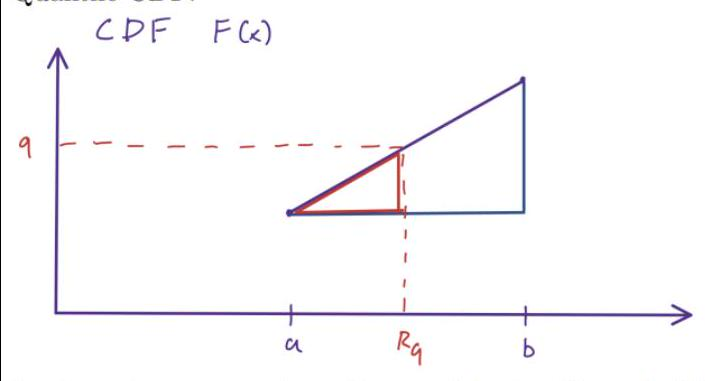
\includegraphics[width=\linewidth]{images/2024_12_29_0906b02acf849bda8665g-1(2)}

Zur Berechnung von $R_{q}$ sucht man diejenige Klasse $[a, b[$ mit $F(a) \leq q \leq F(b) \mathrm{b}$

\begin{itemize}
  \item $m=\frac{q-F(a)}{R_{q}-a}$
  \item $R_{q}=a+(b-a) \cdot \frac{q-F(a)}{F(b)-F(a)}$
  \item $q=F(a)+\frac{F(b)-F(a)}{b-a} \cdot\left(R_{q}-a\right)$
  \item $q=F(a)+f\left(R_{q}\right) \cdot\left(R_{q}-a\right)$
\end{itemize}

\begin{center}
\begin{tabular}{|l|l|l|l|}
\hline
$1!$ & 1 & $6!$ & 720 \\
\hline
$2!$ & 2 & $7!$ & 5040 \\
\hline
$3!$ & 6 & $8!$ & 40320 \\
\hline
$4!$ & 24 & $9!$ & 362880 \\
\hline
$5!$ & 120 & $10!$ & 3628800 \\
\hline
\end{tabular}
\end{center}

Aufgaben

\begin{center}
\begin{tabular}{|c|c|c|c|c|c|}
\hline
\multicolumn{6}{|l|}{Klassierte Daten} \\
\hline
Klasse & AbsH & SummeAbsH & RelH & PDF & CDF \\
\hline
20-30 & 8 & 8 & $\frac{8}{40}$ & $\frac{8}{400}$ & $\frac{8}{40}$ \\
\hline
30-50 & 10 & 18 & $\frac{10}{40}$ & $\frac{10}{800}$ & $\frac{18}{40}$ \\
\hline
50-60 & 18 & 36 & $\frac{18}{40}$ & $\frac{18}{400}$ & $\frac{36}{40}$ \\
\hline
60-80 & 4 & 40 & $\frac{4}{40}$ & $\frac{4}{800}$ & $\frac{40}{40}$ \\
\hline
\end{tabular}
\end{center}

AbsH ->\\
SummeAbsH ->\\
RelH ->\\
P\\
AbsH : (Anzahl * Klassenbreite)\\
CDF\\
Mittelwert

$$
\bar{x}=\frac{1}{40}(25 \cdot 8+40 \cdot 10+55 \cdot 18+70 \cdot 4)=46.75
$$

Varianz\\
$s^{2}=\frac{1}{40}\left(25^{2} \cdot 8+40^{2} \cdot 10+55^{2} \cdot 18+70^{2} \cdot 4\right)-\bar{x}^{2}=190.577$\\
Korrigierte Varianz $\boldsymbol{s}_{\text {korr }}^{2}$

$$
\frac{n}{n-1} \cdot s^{2}=\frac{40}{39} \cdot 190.688=195.577
$$

Standardabweichung $s$

$$
\sqrt{s^{2}}=\sqrt{19.577}=13.809
$$

Korrigierte Standardabweichung $\boldsymbol{S}_{\text {korr }}$

$$
\sqrt{\frac{n}{n-1}} \cdot s=\sqrt{\frac{40}{39}} \cdot 13.809=13.9849
$$

\section*{Median-> $Q_{2}$}
$40 \cdot \frac{1}{2}=20$-> 20 ist in Klasse 50-60 (zwischen 18 - 36)\\
$a=50 b=60$

$$
\begin{gathered}
\mathrm{F}(\mathrm{a})=\frac{18}{40} \quad \mathrm{~F}(\mathrm{~b})=\frac{36}{40} \\
\boldsymbol{R}_{q}=\boldsymbol{a}+(\boldsymbol{b}-\boldsymbol{a}) \cdot \frac{\boldsymbol{q}-\boldsymbol{F}(\boldsymbol{a})}{\boldsymbol{F}(\boldsymbol{b})-\boldsymbol{F}(\boldsymbol{a})}= \\
50+(60-50) \cdot \frac{0.50-\frac{18}{40}}{\frac{36}{40}-\frac{18}{40}}=51.11
\end{gathered}
$$

Interquartilsabstand -> $Q_{3}-Q_{1}$\\
$56.67-34=22.67$\\
$Q_{1}$\\
$40 \cdot \frac{1}{4}=10$-> 10 ist in Klasse 30-50 (zwischen 8 - 18)\\
$\mathrm{a}=30 \mathrm{~b}=50 \quad \mathrm{~F}(\mathrm{a})=\frac{8}{40} \quad \mathrm{~F}(\mathrm{~b})=\frac{18}{40}$

$$
30+(50-30) \cdot \frac{0.25-\frac{8}{40}}{\frac{18}{90}-\frac{8}{40}}=34
$$

$Q_{3}$\\
$40 \cdot \frac{3}{4}=30$-> 30 ist in Klasse 50-60 (zwischen 18 - 36)\\
$\mathrm{a}=50 \mathrm{~b}=60 \quad \mathrm{~F}(\mathrm{a})=\frac{18}{40} \quad \mathrm{~F}(\mathrm{~b})=\frac{36}{40}$

$$
50+(60-50) \cdot \frac{0.75-\frac{18}{40}}{\frac{36}{40}-\frac{18}{90}}=56.67
$$

\section*{Multivariante Statistik}
$[8,-5],[-2,-14],[1,-7]$\\
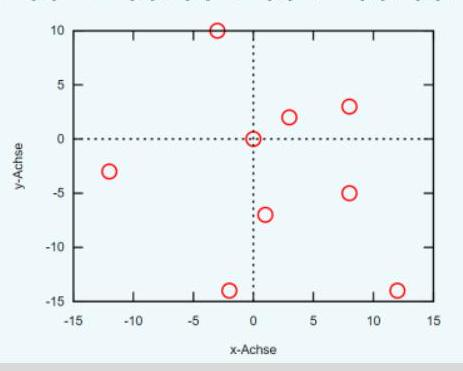
\includegraphics[width=\linewidth]{images/2024_12_29_0906b02acf849bda8665g-1(6)}

\section*{x-Koordinatenliste}
Jeweils erster Wert in den Klammern\\
$[8,-2,1,-12,8,-3,12,0,3]$\\
Sortierte $\mathbf{x}$-Koordinatenliste\\
Einfach sortieren $\rightarrow[-12,-3,-2,0,1,3,8,8,12]$\\
Rangliste $x$-Koordinate\\
Sortierte Liste nehmen und Rangliste erstellen\\
Kommt ein Wert mehrmals vor\\
$\rightarrow$ Ränge addieren und durch Anzahl dividieren\\
$[-12,-3,-2,0,1,3,8,8,12]$\\
$\begin{array}{ccccccc}1 & 2 & 3 & 4 & 5 & 6 & 7\end{array}$\\
Der Wert 8 kommt zwei Mal vor, daher\\
$\frac{7+8}{2} \rightarrow$ Ränge addieren und durch Anzahl dividieren\\
$[-12,-3,-2,0,1,3,8,8,12]$\\
$\begin{array}{lllllllll}1 & 2 & 3 & 4 & 5 & 7.5 & 7.5 & 9\end{array}$\\
Diese Ränge dann in die unsortierte $x$-Koorinatenliste\\
$[8,-2,1,-12,8,-3,12,0,3]$\\
$7.53517 .52 \quad 946 \rightarrow$ Lösung

\section*{y -Koordinatenliste}
Jeweils zweiten Wert in den Klammern\\
$[-5,-14,-7,-3,3,10,-14,0,2]$\\
Sortierte $y$-Koordinatenliste\\
Sortieren $\rightarrow[-14,-14,-7,-5,-3,0,2,3,10]$\\
Rangliste $\boldsymbol{y}$-Koordinate\\
Wie oben $\rightarrow[4,1.5,3,5,8,9,1.5,6,7]$

\section*{Kovarianz (nicht korrigiert)}
Ähnlich zu berechnen wie Varianz\\
$\frac{\sum(x i-\bar{x})(y i-\bar{y})}{n}$\\
$\bar{x}=\frac{8-2+1-12+8-3+12+0+3}{9}=\frac{5}{3}$\\
$\bar{y}=\frac{-5-14-7-3-3+10-14+0+2}{9}=\frac{-34}{9}$\\
$\frac{\left(8-\frac{5}{3}\right)\left(-5+\frac{34}{9}\right)+\left(-2-\frac{5}{3}\right)\left(-14+\frac{34}{9}\right)+\cdots+\left(3-\frac{5}{3}\right)\left(2+\frac{34}{9}\right)}{9}=-11.59$

Pearson Korrelationskoeffizien

\section*{Kovarianz}
$\overline{\text { Standartabweichung } x * \text { Standartabweichung } y}$\\
Taschenrechner $\rightarrow \mathrm{x}$ und y in Tabelle eingeben (benennen) Menu $\rightarrow$ Statistik $\rightarrow$ Stat. Ber. $\rightarrow$ Stat. Mit zwei Var Spalten auswählen, Rest lassen, ok $\rightarrow$ runterscrollen bis «r»

Pearson Korrelationseffizient ist stets im Bereich [0,1]. Desto näher an 1, desto grösser ist die Korrelation.\\
$[-1,0]$ je näher an -1 desto stärker der negative lineare zusammenhang\\
Kovarianz der Ranglisten\\
Gleich wie Kovarianz, nur mit Ranglisten statt normaler Liste Spearman Korrelationskoeffizient\\
Misst die Stärke und Richtung des linearen Zusammenhangs,

$$
\begin{gathered}
r_{x y}=\frac{s_{x y}}{s_{x} \cdot s_{y}} \\
s_{x}=\sqrt{\frac{1}{n} \sum_{i=1}^{n}\left(x_{i}-\bar{x}\right)^{2}}=\overline{x^{2}}-\bar{x}^{2} \\
s_{y}=\sqrt{\frac{1}{n} \sum_{i=1}^{n}\left(y_{i}-\bar{y}\right)^{2}}=\overline{y^{2}}-\bar{y}^{2} \\
s_{x y}=\frac{1}{n} \sum_{i=1}^{n}\left(x_{i}-\bar{x}\right)\left(y_{i}-\bar{y}\right)=\text { Kovarianz }
\end{gathered}
$$

Bsp.:\\
Bsp..

\begin{center}
\begin{tabular}{|c|c|c|c|c|c|c|c|}
\hline
$i$ & 1 & 2 & 3 & 4 & 5 & 6 &  \\
\hline
$x_{i}$ & 59 & 35 & 43 & 23 & 42 & 27 &  \\
\hline
$y_{i}$ & 14.6 & 11.8 & 14.3 & 13.0 & 14.2 & 11.0 &  \\
\hline
$\mathrm{rg}\left(x_{i}\right)$ & 6 & 3 & 5 & 1 & 4 & 2 & $\overline{\operatorname{rg}(x)}$ \\
$=3.5$ &  &  &  &  &  &  &  \\
\hline
$\operatorname{rg}\left(x_{i}\right)-\overline{\operatorname{rg}(x)}$ & 2.5 & -0.5 & 1.5 & -2.5 & 0.5 & -1.5 &  \\
\hline
$\mathrm{rg}\left(y_{i}\right)$ & 6 & 2 & 5 & 3 & 4 & 1 & $\overline{\operatorname{rg}(y)}$ \\
\hline
$\mathbf{3} .5$ &  &  &  &  &  &  &  \\
\hline
$\mathrm{rg}\left(y_{i}\right)-\overline{\operatorname{rg}(y)}$ & 2.5 & -1.5 & 1.5 & -0.5 & 0.5 & -2.5 &  \\
\hline
\end{tabular}
\end{center}

Dabei wird dieser Koeffizient berechnet wie die Pearson-Korrelation mit dem Unterschied, dass $\sum_{i=1}^{n}\left(\operatorname{rg}\left(x_{i}\right)-\overline{\operatorname{rg}(x)}\right)\left(\operatorname{rg}\left(y_{i}\right)-\overline{\operatorname{rg}(y)}\right)$\\
$r_{\text {sp }}=\frac{\sqrt{\sum_{i=1}^{n}\left(\operatorname{rg}\left(x_{i}\right)-\overline{\operatorname{rg}(x)}\right)^{2}} \cdot \sqrt{\sum_{i=1}^{n}\left(\operatorname{rg}\left(y_{i}\right)-\overline{\operatorname{rg}(y)}\right)^{2}}}{2}$\\
$\sum_{i=1}^{n}\left(\operatorname{rg}\left(x_{i}\right)-\overline{\operatorname{rg}(x)}\right)^{2}=\sum_{i=1}^{n}\left(\operatorname{rg}\left(y_{i}\right)-\overline{\operatorname{rg}(y)}\right)^{2}$\\
$=\sqrt{2.5^{2}+(-0.5)^{2}+1.5^{2}+(-2.5)^{2}+0.5^{2}+(-1.5)^{2}}=\sqrt{17.5}$

\section*{CDF Wert berechnen}
In der folgenden Tabelle stehen die PDF Werte einer klassierten Stichprobe:

\begin{center}
\begin{tabular}{|l|c|c|c|c|c|}
\hline
Klassengrenzen & $27-$ & $48-$ & $77-$ & $103-$ & $140-$ \\
\hline
PDF & 48 & 77 & 103 & 140 & 207 \\
\hline
 & $\frac{11}{1281}$ & $\frac{13}{1769}$ & $\frac{4}{793}$ & $\frac{20}{2257}$ & $\frac{9}{4087}$ \\
\hline
\end{tabular}
\end{center}

CDF Wert $\mathrm{F}(153) \rightarrow 153$ ist in der letzten Klasse 207-140 = 67 $\rightarrow 67 * 9=603 \rightarrow 603 / 4087$ in letzter Klasse 4087-603 = $3484 \rightarrow 3484 / 4087$ bis zur letzten Klasse $153-140=13 \rightarrow 13 * 9=117 \rightarrow 117+3484=3061 \rightarrow$ 3061/4087

\section*{PDF Wert berechnen}
\begin{center}
\begin{tabular}{l}
In der folgenden Tabelle stehen die absoluten Haufigkeiten \\
\hline
Klassengrenzen \\
\hline
\end{tabular}
\end{center}

Absolute Häufigkeit \textbackslash begin\{tabular\}\{l|l\}\\
30 \\
\\
14

 \begin{tabular}{cc|c|c|c|}
\end{tabular}

101 \& 209 \& 397 \\
\\
\textbackslash hline 3 \& 11 \& 22 \& 8 \\
\\
\textbackslash hline\\
\textbackslash end\{tabular\}

PDF Wert $\mathrm{f}(759) \rightarrow$ in der letzten Klasse Relative Häufigkeit ausrechnen $\rightarrow 14+3+11+22+8=58$ Letzte Klasse $\rightarrow$ 8/58\\
8/58 ist relative Häufigkeit der ganzen Klasse\\
$\rightarrow$ 839-397 = $442 \rightarrow$ 8/58/442 = 8/25636

\section*{PMF Wert berechnen}
Berechnen Sie den folgenden PMF Wert für die Stichprobe\\
$x=[0,2,-2,-1,3,-2,2,3,0,-1,3,-2,-3,-1,1,2,1,1]$ $f(0)=$ ?\\
Anzahl 0 / Gesamte Anzahl = 2/18\\

\includegraphics[width=\linewidth]{images/2024_12_29_0906b02acf849bda8665g-2} CMF Wert berechnen\\
Berechnen Sie den folgenden CMF Wert für die Stichprobe $x=[-8,1,-2,6,0,1,-8,-2,3,3,3,0,3,-1,3,-2,6,2]$ $F(-3)=$ ?\\
Stichprobe sortieren $\rightarrow$ Anzahl Werte bis gesuchter Wer Im Beispiel $\rightarrow-8,-8$\\
Anzahl Werte / Gesamte Anzahl = 2/18

\section*{Praktikum 1}
\section*{Aufgabe 1}
\section*{Aufabe 1}
a) Bestimmen sie die $P M F$ und CMF der Stichprobe: $X=(-2,10,0,-2,4,-1,3,-2,10,2)$\\
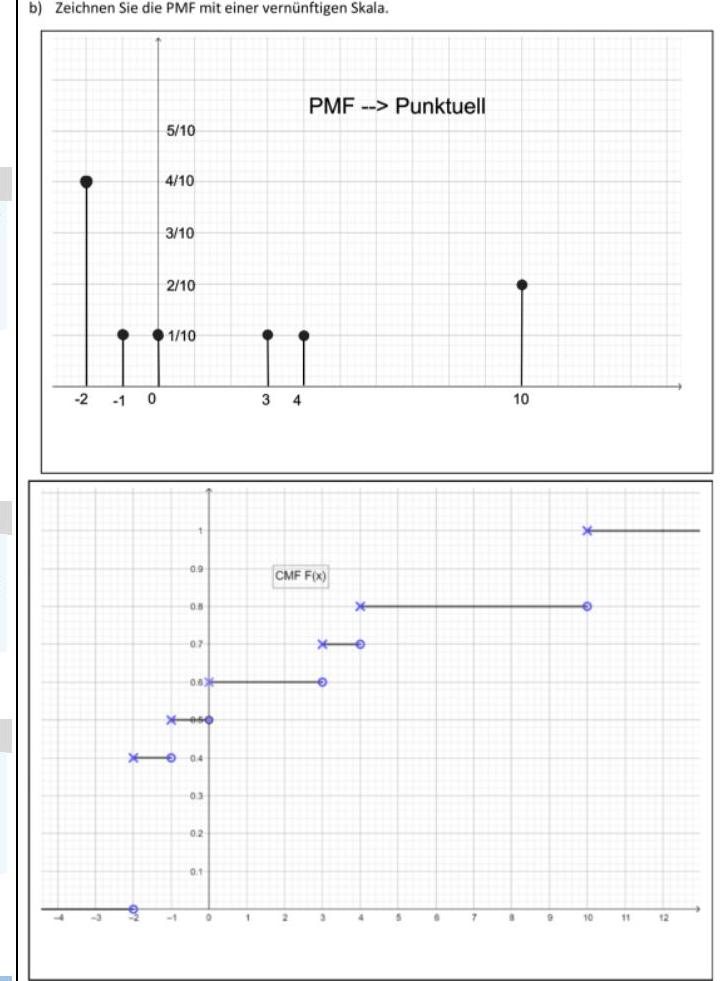
\includegraphics[width=\linewidth]{images/2024_12_29_0906b02acf849bda8665g-2(1)}

\section*{Probleme}
Variation(mit Reihenfolge) - Mit Wiederholung n $\mathbf{n}^{k}$\\
Zahlenschlossproblem:\\
Sie haben den Code ihres 6 stelligem Zahlenschloss(0-9) vergessen. Wie viele Versüche brauchen Sie im schlimmsten\\
Fall?\\
$10^{6}$

\section*{Bitproblem}
Wie viele Zahlen können mit $\mathbf{6 4}$ Bits dargestellt werden? $2^{64}$

\section*{uchstabenproblem:}
Möglichkeiten für 5-Stellige Wörter aus 10\\
Buchstabenplättchen legen:\\
$10{ }^{5}$\\
Variation(mit Reihenfolge) - Ohne Wiederholung Schwimmwettkampf:\\
10 Schwimmer, wie viele Möglichkeiten für das Podest(1-3)\\
gibt es?\\
$\frac{10!}{(10-3)!}$

\section*{Buchstabenproblem:}
Aus Anzahl 5-stelliger Wörtern aus 10 verschiedenen Buchstaben(mehrmals verwendbar):\\
$\frac{10!}{(10-5)!}$

\section*{Generäle:}
Anzahl Möglichkeiten um 11 Generäle um einen runden Tisch zu verteilen:\\
11!\\
General-x immer neben General-y:

\section*{(11-1)!}
Kombination(ohne Reihenfolge) - Mit Wiederholung Zahnarztproblem:\\
3 Spielzeuge ziehen aus 5 Kisten ziehen. Anzahl\\
Möglichkeiten:\\
$\binom{n+k-1}{k}=\binom{7}{3}=35$\\
Tellschiessen:\\
3 Pfeile auf Scheibe mit 10 Bereichen. (+1 daneben) Anzahl Möglichkeiten:\\
$\binom{n+k-1}{k}=\binom{13}{3}=286$\\
Kombination(ohne Reihenfolge) - Ohne Wiederholung Lotto:\\
6 Ziehungen aus 49 Kugeln Chance die richtige kombination zu treffen:\\
$\frac{n!}{(n-k) * k!}=\frac{49}{6}$

Fussballmannschaft:

Die Klasse besteht aus 8 Frauen und 12 Männern. Anzahl Möglichkeiten um im Team 6 Frauen und 5 Männer sind.\\
$\binom{8}{6} \cdot\binom{12}{5}$\\
Teilmengenproblem:\\
Anzahl 3-elementige Teilmengen hat die Menge \{1,2,3,4\}: $\binom{4}{3}=4$\\
Anzahl Teilmengen der Menge \{1,2,3,4\}

Auswahlen von $k$ Objekten aus einer Gesamtheit von $n$ Objekten \begin{tabular}{lll}
Variation (=mit Reihenfolge) & Kombination (=ohne Reihenfolge) &  \\
\hline
Mit Wiedertolung & Ohne Wiederholung & Mit Wiedertolung \\
\hline
\end{tabular}

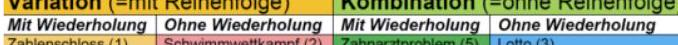
\includegraphics[width=\linewidth]{images/2024_12_29_0906b02acf849bda8665g-3(3)}\\
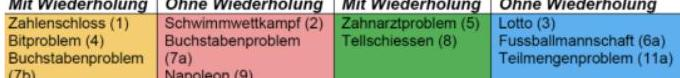
\includegraphics[width=\linewidth]{images/2024_12_29_0906b02acf849bda8665g-3(15)}\\
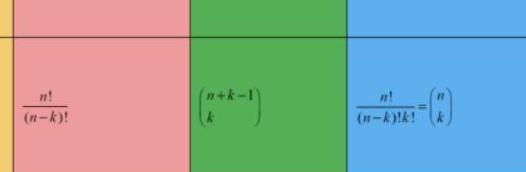
\includegraphics[width=\linewidth]{images/2024_12_29_0906b02acf849bda8665g-3(7)}

\begin{itemize}
  \item Variation von k aus n Objekten mit Wiederholung. - Variation von k aus n Objekten ohne Wiederholung
  \item Kombination von k aus n Objekten mit Wiederholung.
  \item Kombination von k aus n Objekten ohne Wiederholung\\
$\binom{\boldsymbol{n}}{\boldsymbol{k}}->\mathbf{n C r}(\mathbf{n}, \mathbf{k})$\\
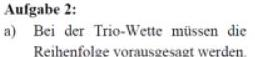
\includegraphics[width=\linewidth]{images/2024_12_29_0906b02acf849bda8665g-3(21)}\\
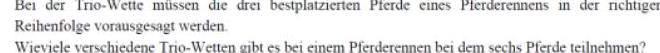
\includegraphics[width=\linewidth]{images/2024_12_29_0906b02acf849bda8665g-3(8)}\\
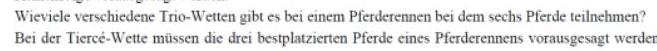
\includegraphics[width=\linewidth]{images/2024_12_29_0906b02acf849bda8665g-3(2)}\\
Die Reikenfolge wird dabei nicht berickscichthigt\\
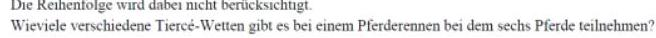
\includegraphics[width=\linewidth]{images/2024_12_29_0906b02acf849bda8665g-3(11)}\\
Losung:
  \item Variation olne Wiedectolung: $\frac{6}{31}=120$ (b) Kombination oline Wiedectolung. $\binom{6}{3}=20$\\
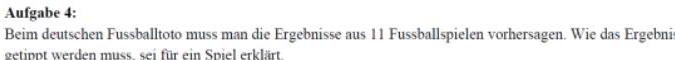
\includegraphics[width=\linewidth]{images/2024_12_29_0906b02acf849bda8665g-3(17)}\\
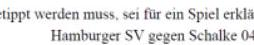
\includegraphics[width=\linewidth]{images/2024_12_29_0906b02acf849bda8665g-3(13)}\\
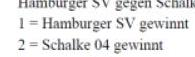
\includegraphics[width=\linewidth]{images/2024_12_29_0906b02acf849bda8665g-3(22)}\\
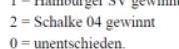
\includegraphics[width=\linewidth]{images/2024_12_29_0906b02acf849bda8665g-3(1)}\\
$0=$ unentschiceden\\
Vie viele mogeliche Tippergebisse gibt es?\\
Lồung\\
Variation\\
range\\
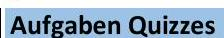
\includegraphics[width=\linewidth]{images/2024_12_29_0906b02acf849bda8665g-3(9)}\\
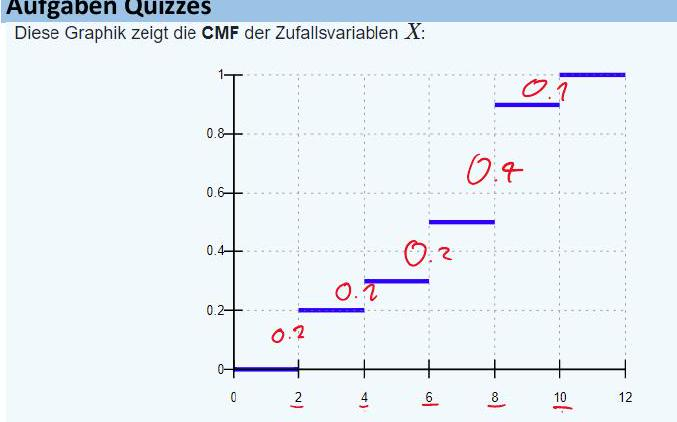
\includegraphics[width=\linewidth]{images/2024_12_29_0906b02acf849bda8665g-3(20)}Bestimmen Sie mithife der Graphik die folgenden Kenngrössen der Zufallsvariablen $X$.\\
$E(X)=6.2 \cdot 0.2+4 \cdot 0.1+6 \cdot 0.2+8 \cdot 0.4+10 \cdot 0.1=6.2$
\end{itemize}

$E\left(X^{2}\right)=45.2 \quad 2^{2} \cdot 0.2+4^{2} \cdot 0.1+6^{2} \cdot 0.2+8^{2} \cdot 0.4+10^{2} \cdot 0.1=45.2$\\
$V(X)=6.76 \quad E\left(X^{2}\right)-E(X)^{2}$

\begin{center}
\begin{tabular}{|c|c|c|c|c|}
\hline
$x$ & 1 & 2 & 3 & 5 \\
\hline
PMF & 0.5 & 0.2 & 0.2 & 0.1 \\
\hline
\end{tabular}
\end{center}

Berechnen Sie die folgenden Kenngrössen:\\
$E(X)=1 \cdot 0.5+2 \cdot 0.2+3 \cdot 0.2+5 \cdot 0.1=2$\\
$E\left(X^{2}\right)=1^{2} \cdot \mathbf{0 . 5 + 2 ^ { 2 } \cdot 0 . 2 + \mathbf { 3 } ^ { 2 } \cdot 0 . 2 + \mathbf { 5 } ^ { 2 } \cdot 0 . 1 = 5 . 6}$\\
$V(X)=E\left(X^{2}\right)-E(X)^{2}=1.6$\\
Anzahl Möglichkeiten einer 6-8 stelligen Zahl mindestens 14 zu haben\\
Auffabe 5:\\
Auf wi cicle\\
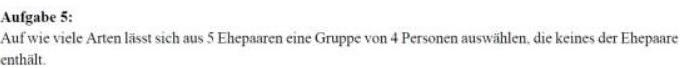
\includegraphics[width=\linewidth]{images/2024_12_29_0906b02acf849bda8665g-3(4)}\\
Lobsung:\\
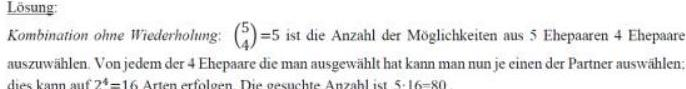
\includegraphics[width=\linewidth]{images/2024_12_29_0906b02acf849bda8665g-3(10)}\\
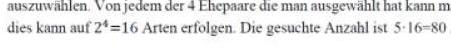
\includegraphics[width=\linewidth]{images/2024_12_29_0906b02acf849bda8665g-3(5)}

\section*{Aulgabe 6}
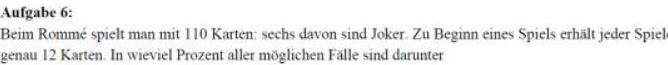
\includegraphics[width=\linewidth]{images/2024_12_29_0906b02acf849bda8665g-3(16)}\\
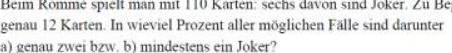
\includegraphics[width=\linewidth]{images/2024_12_29_0906b02acf849bda8665g-3(14)}\\
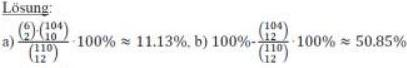
\includegraphics[width=\linewidth]{images/2024_12_29_0906b02acf849bda8665g-3(18)}\\
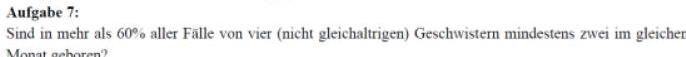
\includegraphics[width=\linewidth]{images/2024_12_29_0906b02acf849bda8665g-3(19)} Monat geboren?\\
$\frac{\text { Losurg. }}{\text { Nein. } 100 \%} \cdot \frac{1211.109}{17^{+}} \cdot 100 \% \approx 42.71 \%$\\
Aurfabe 8:\\
Wic viele W\\
Wie viele Worte lassen sich aus den Buchtsthben des Wortes ABRAKADABRA bilden? (Nur Worte in dene\\
$\frac{\text { Losung }}{\binom{11}{5} \cdot\binom{6}{2} \cdot\binom{4}{4} \cdot\binom{2}{1} \cdot\binom{1}{1}=83160}$\\
Aufgabe 10:\\
Vori inen ste\\
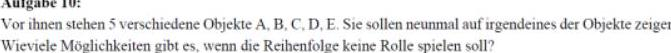
\includegraphics[width=\linewidth]{images/2024_12_29_0906b02acf849bda8665g-3(6)}\\
Losung\\
Kombination mit Wiedecholung. $\binom{5+9-1}{9}=\binom{13}{4}=715$\\
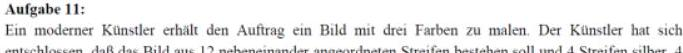
\includegraphics[width=\linewidth]{images/2024_12_29_0906b02acf849bda8665g-3(12)}\\
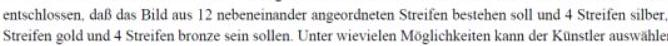
\includegraphics[width=\linewidth]{images/2024_12_29_0906b02acf849bda8665g-3} $\binom{$ Losung \}\{4\}$\cdot\binom{8}{4} \cdot\binom{4}{4}=34650$\\
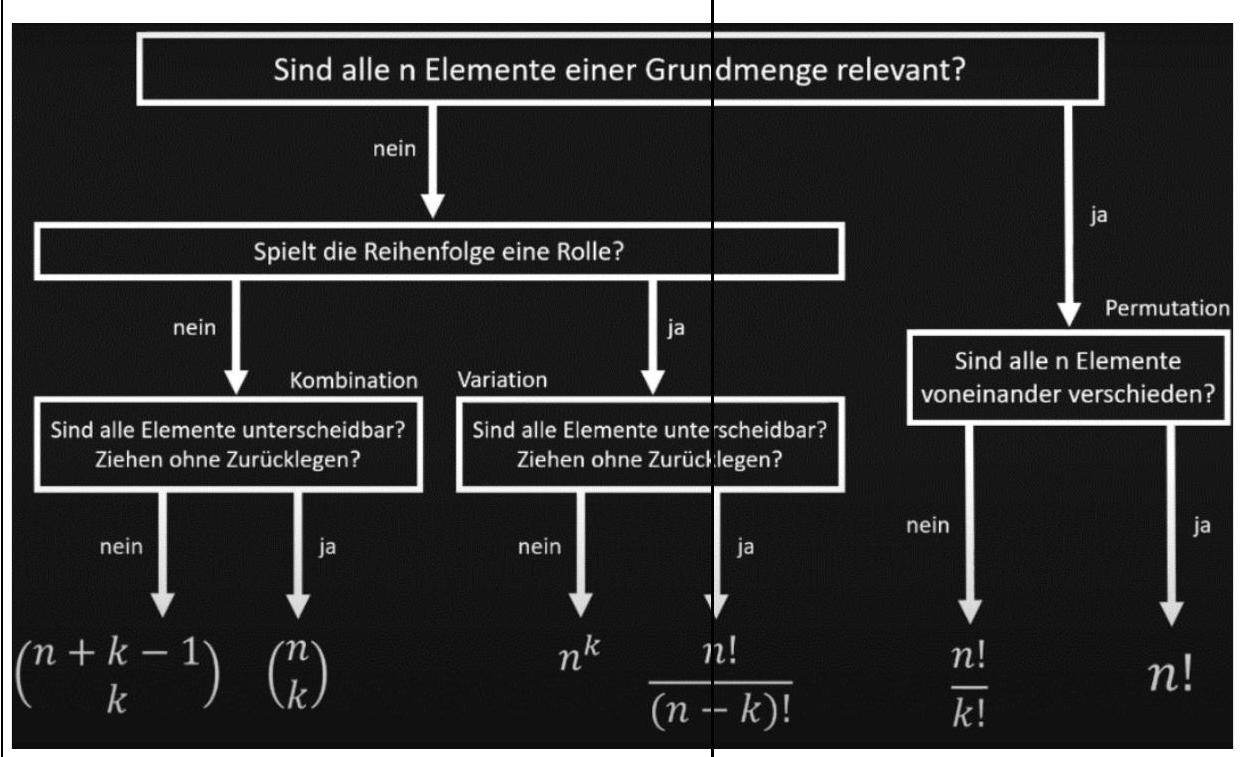
\includegraphics[width=\linewidth]{images/2024_12_29_0906b02acf849bda8665g-3(23)}

\section*{Prüfung 2020}
Prüfung 2020

\begin{center}
\begin{tabular}{|l|c|c|c|c|}
\hline
Aufg 2 &  &  &  &  \\
\hline
 & \begin{tabular}{l}
$[200-$ \\
$400)$ \\
\end{tabular} & \begin{tabular}{l}
$[400-$ \\
$500)$ \\
\end{tabular} & \begin{tabular}{c}
$[500-$ \\
$600)$ \\
\end{tabular} & \begin{tabular}{c}
$[600-$ \\
$1000)$ \\
\end{tabular} \\
\hline
\begin{tabular}{l}
Klassenbreite \\
$b_{i}$ \\
\end{tabular} & 200 & 100 & 100 & 400 \\
\hline
\begin{tabular}{l}
Klassenmitte \\
$m_{i}$ \\
\end{tabular} & 300 & 450 & 550 & 800 \\
\hline
\begin{tabular}{l}
Abs. Häufigk. \\
$h_{i}$ \\
\end{tabular} & 4 & 6 & 8 & 22 \\
\hline
Rel. Häufigk $f_{i}$ & $\frac{4}{40}=0.1$ & $\frac{6}{40}=0.15$ & $\frac{8}{40}=0.2$ & $\frac{22}{40}=0.55$ \\
\hline
\begin{tabular}{l}
Rel. Häufigk \\
dichte(PDF) \\
$f(x)$ \\
\end{tabular} & $\frac{4}{40 \cdot 200}$ & $\frac{6}{40 \cdot 100}$ & $\frac{8}{40 \cdot 100}$ & $\frac{22}{40 \cdot 400}$ \\
\hline
\begin{tabular}{l}
Kummulierte \\
Vert funktion \\
$F(x)$ \\
\end{tabular} & 0.1 & 0.25 & 0.45 & 1 \\
\hline
\end{tabular}
\end{center}

Stichprobenmittel ->\\
$\bar{x}=\Sigma m_{i} \cdot h_{i}=$ Stichprobenvarianz $\boldsymbol{- >} \boldsymbol{s}^{\mathbf{2}}$

$$
s^{2}=\overline{x^{2}}-\bar{x}^{2}=
$$

$\left.300^{2} \cdot 0.1+450^{2} \cdot 0.15+550^{2} \cdot 0.2+800^{2} \cdot 0.55\right)-647.5^{2}$ $=32618.75$\\
Median der klassierten Daten -> $\boldsymbol{Q}_{2}$\\
$40 \cdot \frac{1}{2}=20$-> 20 ist in Klasse 600-1000 (zwischen 0.45 - 1) $a=600 b=1000 \quad F(a)=0.45 \quad F(b)=1$\\
$R_{0.5}=600+(1000-600) \cdot \frac{0.5-0.45}{1-0.45}=\mathbf{6 3 6 . 3 6 4}$

\section*{Boxplot 1 Aufg}
Daten: $\{2700,2850,2930,3040,2600,4160\} n=6$\\
Sortiert: $\{2600,2700,2850,2930,3040,4160\}$\\
$Q_{1}$\\
2700\\
$\mathbf{Q}_{285}$\\
$\frac{2850+2930}{2}=2890$\\
$\mathrm{Q}_{3}$\\
IQR * 1.5\\
$I Q R \cdot 1.5=Q_{3}-Q_{1}=340 \cdot 1.5=\mathbf{5 1 0}$\\
Untere Antenne (alles zwischen Q1 bis Q1-510)\\
2600\\
Obere Antenne (alles zwischen Q3 bis Q3+510)\\
keine\\
Unterer Ausreisser - keine\\
Oberer Ausreisser\\
4160\\
Boxplot\\
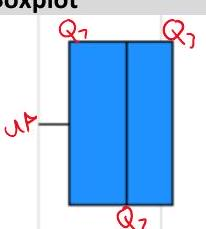
\includegraphics[width=\linewidth]{images/2024_12_29_0906b02acf849bda8665g-4(6)}

Ausreisser

$$
\text { Aufg } 4
$$

\begin{center}
\begin{tabular}{|l|}
\hline
Aufg 4 \\
\hline
Tag $i$ \\
\hline
\end{tabular}
\end{center}

\begin{center}
\begin{tabular}{|l|c|c|c|c|c|c|}
\hline
Tag $i$ & 1 & 2 & 3 & 4 & 5 & Mittelwert \\
\hline
Preis $x_{i}$ & 4.7 & 4.3 & 3.8 & 4.5 & 5.2 & 4.5 \\
\hline
Tagesmenge $y_{i}$ & 70 & 75 & 80 & 75 & 50 & 70 \\
\hline
\end{tabular}
\end{center}

\begin{center}
\begin{tabular}{|l|l|l|l|l|}
\hline
Pearson-Korrelationskoeffizient 1. &  &  &  \\
\hline
$\operatorname{Tag} i$ & 1 & 2 & 3 \\
\hline
\end{tabular}
\end{center}

\begin{center}
\begin{tabular}{|l|c|c|c|c|c|c|}
\hline
Tag $i$ & 1 & 2 & 3 & 4 & 5 & Mittelwert \\
\hline
Preis $x_{i}$ & 4.7 & 4.3 & 3.8 & 4.5 & 5.2 & 4.5 \\
\hline
Tagesmenge $y_{i}$ & 70 & 75 & 80 & 75 & 50 & 70 \\
\hline
$x_{i}^{2}$ & 22.09 & 18.49 & 14.44 & 20.25 & 27.04 & 20.462 \\
\hline
$y_{i}^{2}$ & 4900 & 5625 & 6400 & 5625 & 2500 & 5010 \\
\hline
\end{tabular}
\end{center}

$$
s_{x y}=\overline{x y}-\bar{x} \bar{y}=310.6-4.5 \cdot 70=-4.40
$$

$$
r_{x y}=\frac{s_{x y}}{s_{x} s_{y}}=\frac{-4.5}{\sqrt{0.212} \cdot \sqrt{0}}
$$

$$
\frac{-4.5}{2 \cdot \sqrt{0.110}}
$$

$$
\overline{\overline{10}}=-0.911
$$

$\rightarrow \quad-0.911=$ starker negativer Zusammenhang zwischen Tagesmenge und Preis

\section*{Pearson-Korrelationskoeffizient 2}
Kovarianz\\
Standartabweichung $x *$ Standartabweichung $y$

$$
k o v=\frac{\sum(x i-\bar{x})(y i-\bar{y})}{n}
$$

$$
s_{x}^{2}=\frac{1}{n} \sum_{i=1}^{n}\left(x_{i}-\bar{x}\right)^{2}
$$

$$
s_{x}=\sqrt{s_{x}^{2}}
$$

Lineare regression in $y$ Richtung

$$
m=\frac{s_{x y}}{s_{x}^{2}}=\frac{-4.40}{0.212}=-20.755
$$

$d=\bar{y}-m \bar{x}=70-(-20.755) \cdot 4.5=163.40$\\
$\rightarrow$ Zunahme des Preises um 1CHF/kg senkt verkauf um $20.755 \mathrm{~kg} / \mathrm{d}$

\section*{Bestimmtheitsmas}
$$
R^{2}=r_{x y}^{2}=-0.911^{2}=0.8299
$$

82.99\% der Gesamtvarianz in den yDaten kann durch die regressionsgerade erklärt werden.\\
Preis damit $90 \mathrm{~kg} / \mathrm{d}$ verkauft werden

$$
\begin{gathered}
\hat{y}=90 \Rightarrow \quad \hat{\boldsymbol{x}}=\frac{\mathbf{1}}{n}(\widehat{y}-d) \\
=\frac{\mathbf{1}}{-\mathbf{2 0 . 7 5 5}} \cdot(\mathbf{9 0}-\mathbf{1 6 3 . 4 0})=3.54 \mathrm{CHF}
\end{gathered}
$$

\section*{Aufg 5}
Aufg 5 abgebildet Ticket wird mit e einem Slannmuster entwertet.\\
a) (1 Punkt) Dabei werden bei der Entwertung drei Löcher in die neun Felder des\\
Tickets gestanzt. Wie viele solcher Karten musste man sammeln, um alle

Irickets gestannt. Wie viele solcher Karten müsste man sammeln, um allc\\
möglichen Stanzmuster rub besitzen?\\
(2 Punkte) U. dier and\\
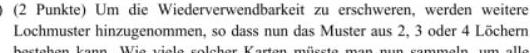
\includegraphics[width=\linewidth]{images/2024_12_29_0906b02acf849bda8665g-4(7)} bestehen kann. Wie viele solcher Kar\\
möglichen Stanzmuster zu besitzen?\\
Um einem Betruy voraubecugen wird nun neu statdessen cin Code auf die Karte gestempelt.\\
Wie vieles solcher Karten müste man nun sammeln,\\
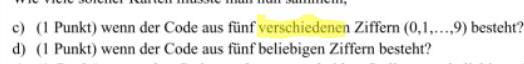
\includegraphics[width=\linewidth]{images/2024_12_29_0906b02acf849bda8665g-4}\\
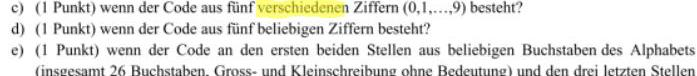
\includegraphics[width=\linewidth]{images/2024_12_29_0906b02acf849bda8665g-4(3)}\\
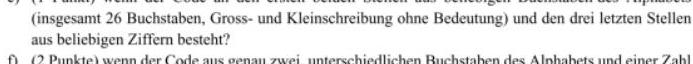
\includegraphics[width=\linewidth]{images/2024_12_29_0906b02acf849bda8665g-4(5)}\\
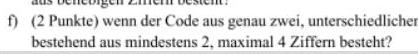
\includegraphics[width=\linewidth]{images/2024_12_29_0906b02acf849bda8665g-4(4)}\\
a)\\
$\binom{n}{k}=\binom{9}{3}=84$

$$
\begin{aligned}
& s_{x}^{2}=\overline{x^{2}}-\bar{x}^{2}=20.462-4.5^{2}=0.212 \\
& s_{y}^{2}=\overline{y^{2}}-\bar{y}^{2}=5010-70^{2}=110
\end{aligned}
$$

\begin{center}
\begin{tabular}{|c|c|c|c|}
\hline
\multicolumn{4}{|l|}{b)} \\
\hline
\multicolumn{4}{|c|}{$\binom{9}{2}+\binom{9}{3}+\binom{9}{4}=246$} \\
\hline
\multicolumn{4}{|l|}{c)} \\
\hline
\multicolumn{4}{|c|}{$\overline{(n-k)!}=\overline{(10-5)!}=30240$} \\
\hline
\multicolumn{4}{|l|}{d)} \\
\hline
\multicolumn{4}{|c|}{$10 \cdot 10 \cdot 10 \cdot 10 \cdot 10=100^{\prime} 000$} \\
\hline
\multicolumn{4}{|l|}{e)} \\
\hline
\multicolumn{4}{|c|}{$26 \cdot 26 \cdot 10 \cdot 10 \cdot 10=676^{\prime} 000$} \\
\hline
\multicolumn{4}{|l|}{f)} \\
\hline
\multicolumn{4}{|c|}{$26 \cdot 25 \cdot\left(10^{2}+10^{3}+10^{4}\right)=7^{\prime} 215^{\prime} 000$} \\
\hline
\multicolumn{4}{|l|}{Aufg 6} \\
\hline
\multicolumn{4}{|l|}{\multirow[t]{4}{*}{\begin{tabular}{l}
Roche hat einen «Rapid Antigen Tests, herausgegeben, mit welchem man eine akute EFrrankung an SARS-Cov-2 nachwcisen kann. \\
Die Firma schreibt, dass der Test eine an SARS-Cov-2 erkrankte Person mit einer Wahrscheinlichkeit von $96.52 \%$ korrekt als an der Krankheit erkrankt diagnostiziert (Testergebnis positiv, gegeben dass die Person atsächlich erkrankt ist). \\
Eine gesunde Person wird mit einer Wahrscheinlichkeit von $99.68 \%$ als gesund erkannt (Testergebnis negativ, gegeben dass die Person tatsächlich gesund ist). \\
In dieser Aufgabe gehen wir davon aus, dass in einer Region mit ca. $1^{\prime} 000^{\prime} 000$ Einwohnern $1 \%$ aktuell an \\
Covid 19 erkrankt sind und die Angaben der Firma zutreffen. \\
a) \\
\end{tabular}}} \\
\hline
 &  &  &  \\
\hline
 &  &  &  \\
\hline
 &  &  &  \\
\hline
\multicolumn{4}{|l|}{(3) Punkte) Befullen Sie die untenstehende Kontingentabelle (graue Felder) miid den genannten Zahlen.} \\
\hline
 & Testergebis positiv & Testergebnis negativ &  \\
\hline
\multicolumn{4}{|l|}{Akut cekrankt} \\
\hline
\multicolumn{4}{|l|}{\multirow[t]{2}{*}{Akut nicht erkrankt}} \\
\hline
 &  &  &  \\
\hline
 & Test positiv & Test negativ &  \\
\hline
Akut krank & 9652 & 348 & 10 '000 \\
\hline
Nicht krank & 3168 & 986 '832 & 990'000 \\
\hline
 & 12820 & 987'180 & 1'000'000 \\
\hline
b) &  &  &  \\
\hline
\end{tabular}
\end{center}

b) $(1$ Punk) Wie gross ist die Wahrscheinlichkeit, dass e eine Person akut an SARS-Cov-2 erkrankt ist und\\
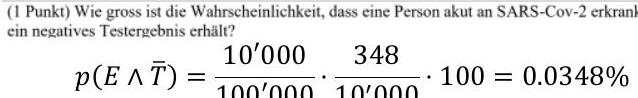
\includegraphics[width=\linewidth]{images/2024_12_29_0906b02acf849bda8665g-4(2)}\\
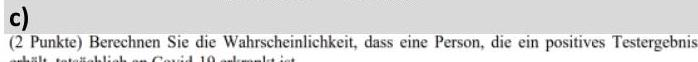
\includegraphics[width=\linewidth]{images/2024_12_29_0906b02acf849bda8665g-4(9)} (2 Punkte) Berechnen Sie die Wahrsche\\
challt, tatsachchlich an Covid-19 erkrankt is

$$
p(E \wedge T \mid T)=\frac{9652}{12^{\prime} 820} \cdot 100=75.29 \%
$$

d) $\quad P($ Erkrankt $)=1 \%$

$$
P(\text { Positiv })=1.282 \%
$$

$$
P(E P)=\frac{9652}{10000}=0.97
$$

$$
P(E P) \neq P(E) * P(p)
$$

$==$ Nicht stochastisch unabhängig!

\section*{Aufgabe 8}
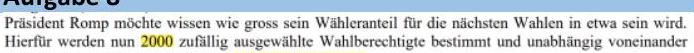
\includegraphics[width=\linewidth]{images/2024_12_29_0906b02acf849bda8665g-4(1)}\\
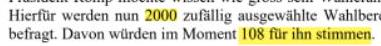
\includegraphics[width=\linewidth]{images/2024_12_29_0906b02acf849bda8665g-4(10)}\\
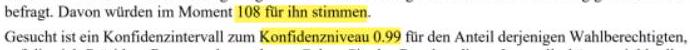
\includegraphics[width=\linewidth]{images/2024_12_29_0906b02acf849bda8665g-4(11)}\\
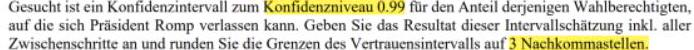
\includegraphics[width=\linewidth]{images/2024_12_29_0906b02acf849bda8665g-4(8)} $\hat{p}=\frac{108}{2000}$\\
$q=\frac{1+y}{2}=\frac{1+0.99}{2}=0.995$\\
$\mathrm{c}=0.975$ aus Tabelle: $\mathrm{u}_{\mathrm{p}}$ aus Liste $->2.576$

$$
\begin{aligned}
\bar{x} & =\hat{p} \\
\theta_{u} & =\bar{x}-c \cdot \sqrt{\frac{\bar{x} \cdot(1-\bar{x})}{n}} \\
\theta_{o} & =\bar{x}+c \cdot \sqrt{\frac{\bar{x} \cdot(1-\bar{x})}{n}}
\end{aligned}
$$

Von 0.041-0.067\\
$2600 \quad 3000 \quad 3400 \quad 3800 \quad 4200$\\
Affoltere Gang\\
Prüfung 2018

\begin{center}
\begin{tabular}{|l|l|l|}
Aufg 1 &  &  \\
\hline
\begin{tabular}{l}
X \\
von...bis.. \\
\end{tabular} & \begin{tabular}{l}
Absolute \\
Häufigkeit $h_{i}$ \\
\end{tabular} & \begin{tabular}{l}
Relative Summen- \\
häufigkeit $F_{i}(C D F)$ \\
\end{tabular} \\
\hline
$200-500$ & 600 & $\frac{600}{1500}=0.4$ \\
\hline
$500-600$ & 300 & $\frac{900}{1500}$ \\
\hline
$600-800$ & 100 & $\frac{1000}{1500}$ \\
\hline
$800-1000$ & 500 & $\frac{1500}{1500}$ \\
\hline
\end{tabular}
\end{center}

\subsection*{0.3 Quanti}
$\frac{0.4}{500-200}=\frac{0.3}{R_{0.3}-200} \rightarrow R_{0.3}=\frac{500-200}{0.4} \cdot 0.3+200=\mathbf{4 2 5}$ $500-200$\\
$\%<=880$

$$
\begin{gathered}
600+300+100+\left(\frac{500}{200} \cdot 80\right)=1200 \\
\frac{100 \cdot 1200}{1500}=\mathbf{8 0} \%
\end{gathered}
$$

\section*{Aufg 2}
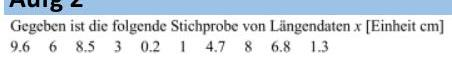
\includegraphics[width=\linewidth]{images/2024_12_29_0906b02acf849bda8665g-5(15)}\\
Klassieren Sie die Daten in 3 aneinander liegende Klassen 1,1, und III, so dass die uygehörigen PDF und die CDF Werte die folgende Tabelle e crillen:\\
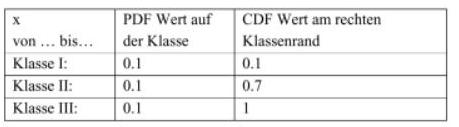
\includegraphics[width=\linewidth]{images/2024_12_29_0906b02acf849bda8665g-5(2)}\\

\includegraphics[width=\linewidth]{images/2024_12_29_0906b02acf849bda8665g-5(13)}\\
Gegeben ist die folgende Stichprobe von Längendaten $x$ [Einheit cm] $\begin{array}{llllllllll}9.6 & 6 & 8.5 & 3 & 0.2 & 1 & 4.7 & 8 & 6.8 & 1.3\end{array}$ Klassieren Sie die Daten in 3 aneinander liegende Klassen I, II, und III, so dass die zugehörigen PDF und die

\section*{CDF Werte die folgende Tabelle erfüllen:}
CDF Werte die folgende Tabelle erfüllen:

\begin{center}
\begin{tabular}{|l|l|l|}
\hline
\begin{tabular}{l}
X \\
von $\ldots$ bis $\ldots$ \\
\end{tabular} & \begin{tabular}{l}
PDF Wert auf \\
der Klasse \\
\end{tabular} & \begin{tabular}{l}
CDF Wert am rechten \\
Klassenrand \\
\end{tabular} \\
\hline
Klasse I: & 0.1 & 0.1 \\
\hline
Klasse II: & 0.1 & 0.7 \\
\hline
Klasse III: & 0.1 & 1 \\
\hline
\end{tabular}
\end{center}

\section*{Stichprobe ordnen}
$0,211.334 .766 .888 .59 .6$\\
Klassenbreite $=\frac{\text { CDF der Klasse }}{\text { PDF der Klasse }}$\\
Klasse 1 $=\frac{0.1}{0.1}=1$\\
Klasse 2 $=\frac{0.6}{0.1}=6$\\
Klasse $3=\frac{0.3}{0.1}=3$\\
0,2||1 $1.334 .766 .8 \mid 8$ 8.5 9.6 $\rightarrow$ Klassengrenzen Mögliche Klassengrenzen\\
$I=[0,1[, \quad I I=[1,7[, \quad I I I=[7,10$

\section*{Aufg 3-Boxplot}
$X=\{2,-1,3,4,9,4,-1,2,2\}$\\
X\_sort $=\{-1,-1,2,2,2,3,4,4,9\}$\\
Q1\\
$Q_{1}=\frac{-1+2}{2}=0.5$\\
Q2 - Median\\
$Q_{2}=2$\\
Q3\\
$Q_{1}=\frac{4+4}{2}=4$

IQR 1.5\\
$I Q R \cdot 1.5=\left(Q_{3}-Q_{1}\right) \cdot 1.5=(4-0.5) \cdot 1.5=5.25$ Untere Antenne\\
$0.5-5.25=-4.75->-1$\\
Obere Antenne\\
$4+5.25=9.25$-> 9\\
Untere Ausreisser - keine\\
Obere Ausreisser - keine\\
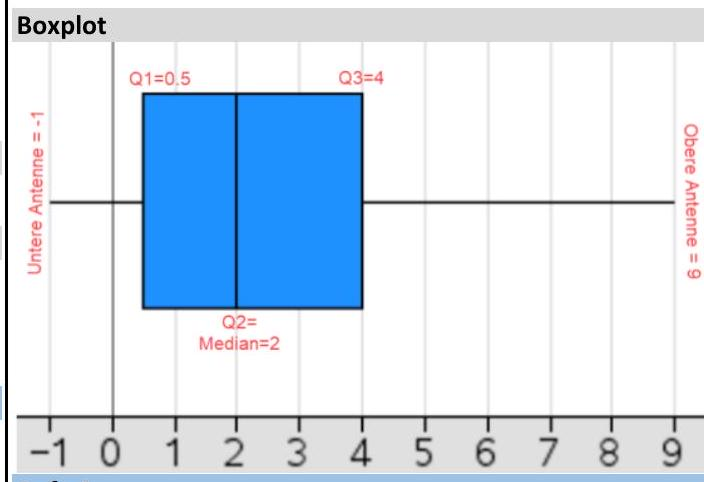
\includegraphics[width=\linewidth]{images/2024_12_29_0906b02acf849bda8665g-5(16)}

\section*{Aufg 4}
\includegraphics[width=\linewidth]{images/2024_12_29_0906b02acf849bda8665g-5(12)}\\
\includegraphics[width=\linewidth]{images/2024_12_29_0906b02acf849bda8665g-5(14)}\\
a) Skizieren Sie einen Scaterplot der Daten, Wie interpreteren Sie diesen Plot? (2 Punkte)\\
\includegraphics[width=\linewidth]{images/2024_12_29_0906b02acf849bda8665g-5(11)}

Ein leichter linearer (positiver) Zusammenhang besteht zwischen Aufwand und Note.\\
b) Bestimme arithmetische Mittel und die Varianz von

\section*{Aufwand und Note sowie die Kovarianz (inkl. Tabelle)}
\includegraphics[width=\linewidth]{images/2024_12_29_0906b02acf849bda8665g-5(7)}\\
$V(A)=\overline{A^{2}}-\bar{A}^{2}=121-\left(\frac{51}{5}\right)^{2}=16.96$\\
$V(N)=\overline{N^{2}}-\bar{N}^{2}=25.5-5^{2}=0.5$\\
$\operatorname{Kov}(A, N)=\overline{A N}-\bar{A} \cdot \bar{N}=52.5-\frac{51}{5} \cdot 5=1.5$\\
c) Berechne den Korrelationskoeffizienten. Was bedeutet dies? Was würden Sie den Studierenden empfehlen?

$$
r_{A, N}=\frac{\operatorname{Kov}(A, N)}{\sqrt{V(A)} \cdot \sqrt{V(N)}} \approx \frac{1.5}{9.2087 \cdot 0.7071}=0.51
$$

Leichter linearer Zusammenhang besteht. Nach dem\\
Bestimmtheitsmass $R^{2}=r_{A, N}{ }^{2} \approx 0.2652$ sind etwa $27 \%$ der auftretenden $N$ Werte durch die linear prognostizierten N Werte erklärt. Viel arbeiten!

\section*{Aufgabe 5}
Gegeben: 5 Programme -> Anz Auswahlen z.B.(P1, P3, P5) von MINDESTENS 2 gibt es\\
$\binom{5}{5}+\binom{5}{4}+\binom{5}{3}+\binom{5}{2}=26$ oder $2^{5}-\binom{5}{1}-\binom{5}{0}=26$\\
Die 5 Programme werden nacheinander ausgeführt. Wie viele verschiedene reihenfolgen gibt es?\\
$5!=120$\\
Zu jeder Kombination aus Programmen hintereinander von mind 1 Programm wird zu jeder Möglichkeit ein test generiert. Wie viele solche Tests gibt es?\\
$\frac{5!}{(5-1)!}+\frac{5!}{(5-2)!}+\frac{5!}{(5-3)!}+\frac{5!}{(5-4)!}+\frac{5!}{(5-5)!}=325$ $\mathbf{2}$ von den 5 programmen sind jetzt identisch, wie sehen die 3 berechnungen jetzt aus?

$$
\begin{aligned}
& \text { a) }\binom{4}{4}+\binom{4}{3}+\binom{4}{2}=11 \\
& \text { b) }\binom{5}{2} * 3!=10 * 6=60
\end{aligned}
$$

c) Es gibt 4 unterschiedliche Fälle

7n a) $\sum_{k=1}^{4}\binom{4}{k}=2^{4}-\sum_{k=0}^{1}\binom{4}{k}=16-\binom{4}{0}-\binom{4}{1}=16-1-4=11$\\
zub) $\binom{5}{2} 3!=10 \cdot 6=60$\\
zu c) 4 Falle:\\
A) Auswahlen ohe Pl und ohne P2:\\
$\sum_{k=1}^{3}\binom{3}{k} \cdot k!=\sum_{k=1}^{3} \frac{3!}{(3-k): k!} \cdot k!=\sum_{k=1}^{3} \frac{3!}{(3-k)!}=3+6+6=15$\\
B) Auswahlen obnc P1 und mit P2:\\
$\sum_{k=0}^{3}\binom{3}{k} \cdot(k+1)!=\sum_{k=0}^{3} \frac{3!}{(3-k)!k!} \cdot(k+1)!=3!\sum_{k=0}^{3} \frac{(k+1)}{(3-k)!}=1+6+18+24=49$\\
C) Auswahlen mit P1 und othe P2: wie Fall B), ergibd diesestben Reihenfolgen, da P1 und P2 identis

C Auss\\
sind.\\
D) Aus\\
D) Auswahlen mit Pl und mit P2, d.h. zweimal dasselbe Programm\\
$\sum_{k=0}^{3}\binom{3}{k} \cdot k!\binom{2+k}{2}=\sum_{i=0}^{3} \frac{3!}{(3-k)!k!} \cdot k!\frac{(2+k)!}{2!k!}=\sum_{k=0}^{3} \frac{3 \cdot(2+k)!}{(3-k)!k!}=3\left(\frac{1}{3}+3+12+20\right)=106$

\section*{Total erhall man: $15+49+106=170$}
\section*{Aufgabe 6}
Datenpaket aus 4 Ubertragungsbits und 2 Korrekturbits.\\
Jedes Bit mit Wahrscheinlichkeit p fehlerhaft.\\
Ein korrektes Korrekturbit kann ein fehlerhaftes\\
Übertragungsbit korrigieren, ein fehlerhaftes Korrekturbit jedoch nicht.\\
Bits sind voneinander stochastisch unabhängig.\\
Ein Paketfehler tritt auf, wenn mind. 1 Bit fehlerhaft ist. Berechne die Paketfehlerwahrscheinlichkeit.

K = Anzahl korrekter Korrekturbits

$$
P(U=k)=\binom{4}{k}(1-p)^{k} * p^{4-k}
$$

Und

$$
P(K=n)=\binom{2}{n}(1-p)^{n} * p^{2-n}
$$

$P($ korrektes Paket $)=P(U=4)+P(U=3)$ $+6(1-p)^{2} p^{2}(1-p)^{2}$\\
rektes Paket)\\
$\mathrm{P}($ Paketfehler $)=1-P($ korrektes Paket $)$

\section*{Aufgabe 7}
2 Runden, fairer 6-seitiger Würfe

\begin{enumerate}
  \item Runde = Win bei 1-3 / Loose bei 4-6
\end{enumerate}

Wenn Win in 1. Runde: 2. Runde gleiche Chancen\\
Wenn Loose in 1. Runde: 2 . Runde $=1-4=$ Win $/ 5-6=$ Loose R1 $=$ G und R2 $=\mathrm{G} \rightarrow$ Gewinn\\
$\mathrm{R} 1=\bar{G}$ und $\mathrm{R} 2=\bar{G} \rightarrow$ Verloren\\
a) Erstelle Wahrscheinlichkeitstabelle

\begin{center}
\begin{tabular}{|c|c|c|}
\hline
 & $R_{2}=G$ & $R_{2}=\bar{G}$ \\
\hline
$R_{1}=G$ & $1 / 4$ & $1 / 4$ \\
\hline
$R_{1}=\bar{G}$ & $1 / 3$ & $1 / 6$ \\
\hline
\end{tabular}
\end{center}

b) Erstelle Tabelle mit Randwahrscheinlichkeiten

\begin{center}
\begin{tabular}{|c|c|c|c|}
\hline
 & $R_{2}=G$ & $R_{2}=\bar{G}$ & $P D F$ von $R_{1}$ \\
\hline
$R_{1}=G$ & $1 / 4$ & $1 / 4$ & $1 / 2$ \\
\hline
$R_{1}=\bar{G}$ & $1 / 3$ & $1 / 6$ & $1 / 2$ \\
\hline
$P D F$ von $R_{2}$ & $7 / 12$ & $5 / 12$ & 1 \\
\hline
\end{tabular}
\end{center}

Sind R1 = G und R2 = G abhängig oder unabhängig?\\
Die beiden Ereignisse sind stochastisch abhängig, denn z.B.:\\
$P\left(R_{1}=G \wedge R_{2}=G\right)=\frac{1}{4} \neq \frac{1}{2} \cdot \frac{7}{12}=P\left(R_{1}=G\right) \cdot P\left(R_{2}=G\right)$

\section*{Aufgabe 8}
\includegraphics[width=\linewidth]{images/2024_12_29_0906b02acf849bda8665g-5(9)}\\
\includegraphics[width=\linewidth]{images/2024_12_29_0906b02acf849bda8665g-5(8)}\\
\includegraphics[width=\linewidth]{images/2024_12_29_0906b02acf849bda8665g-5(3)}\\
\includegraphics[width=\linewidth]{images/2024_12_29_0906b02acf849bda8665g-5(6)}\\
\includegraphics[width=\linewidth]{images/2024_12_29_0906b02acf849bda8665g-5(5)}\\
\includegraphics[width=\linewidth]{images/2024_12_29_0906b02acf849bda8665g-5(1)} Ereignisse: 11 : Fahrzeng vom Typl, T2: Fahrzeuly vom Typl, F1: Fehler bei erster Testah\\
F2: Fehler bei iweiter Testahnt.\\
$P(T 1)=\frac{1}{6}, P(T 2)=\frac{5}{6}, P(\neg F 1 \mid T 1)=0.98, P(\neg F 1 \mid T 2)=0.75$\\
$P(T 1 \mid \neg F 1 \wedge \neg F 2)=\frac{P(T 1 \wedge \neg F 1 \wedge \neg F 2)}{P(\neg F 1 \wedge \neg F 2)}=\frac{\frac{1}{6} \cdot 0.98^{2}}{\frac{1}{6} \cdot 0.98^{2}+\frac{5}{6} \cdot 0.75^{2}} \approx 0.255$\\
b) Bestimme Wahrscheinlichkeit, dass 3. Fahrt auch fehlerlos\\
$P(\neg F 3 \mid \neg F 1 \wedge \neg F 2)=\frac{P(\neg F 1 \wedge \neg F 2 \wedge \neg F 3)}{P(\neg F 1 \wedge \neg F 2)}=\frac{\frac{1}{6} \cdot 0.98^{3}+\frac{5}{6} \cdot 0.75^{3}}{\frac{1}{6} \cdot 0.98^{2}+\frac{5}{6} \cdot 0.75^{2}} \approx 0.81$

$$
\begin{aligned}
& *(P(K=1)+P(K=2)) \\
&+P(U=2) * P(K=2) \\
&=(1-p)^{4}+4(1-p)^{3} p\left(2(1-p) p+(1-p)^{2}\right) \\
&+6(1-p)^{2} p^{2}(1-p)^{2}
\end{aligned}
$$

b) E\\
\includegraphics[width=\linewidth]{images/2024_12_29_0906b02acf849bda8665g-5(17)}\\
\includegraphics[width=\linewidth]{images/2024_12_29_0906b02acf849bda8665g-5}

\section*{-}
\begin{itemize}
  \item 
\end{itemize}

的的

\section*{\begin{center}
\includegraphics[width=\linewidth]{images/2024_12_29_0906b02acf849bda8665g-5(10)}
\end{center}}
\begin{center}
\includegraphics[width=\linewidth]{images/2024_12_29_0906b02acf849bda8665g-5(4)}
\end{center}


\end{document}